\chapter{First iteration}
\label{chap:first-iteration}
In this chapter the first iteration is discussed. The first iteration included the initial analysis and design in which two different design models will be shown: The first theoretical design and the actual design. Afterwards the fruition of the design will be discussed in the implementation segment. Lastly an evaluation of the iteration, which deals with the issues of the current application and how to improve it in the next iteration.

\section{Analysis and Design}
\subsection{The SPARQL object}
As SPARQL is the main essence of the project, the SPARQL class will be the primary focus of the design. The principle of the SPARQL class is to implement essential functionality of a SPARQL query. This means that it should be possible to take a given SPARQL query and break it down into this class form. With this class, SPARQL objects can be created, which can be sent as a common ground between the visual and the textual parsers. A simplistic overview of the relation can be seen in \ref{fig:sparql-interaction} below.
\begin{figure}[h]
    \centering
    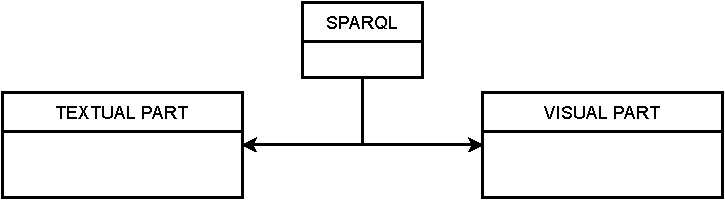
\includegraphics[width=1\textwidth]{figures/sparql-interaction.pdf}
    \caption{Simplistic overview of the relationship between the parsers and the SPARQL class}
    \label{fig:sparql-interaction}
\end{figure}

\subsection{From Query to class}
As the focus of the project is to implement simple queries into the system, select queries have been the heart of the SPARQL class.  By using the SPARQL query in figure \ref{fig:sparql-example}, the following class diagram is created, figure \ref{fig:SPARQL-Triple-class}

\begin{figure}[H]
    \centering
    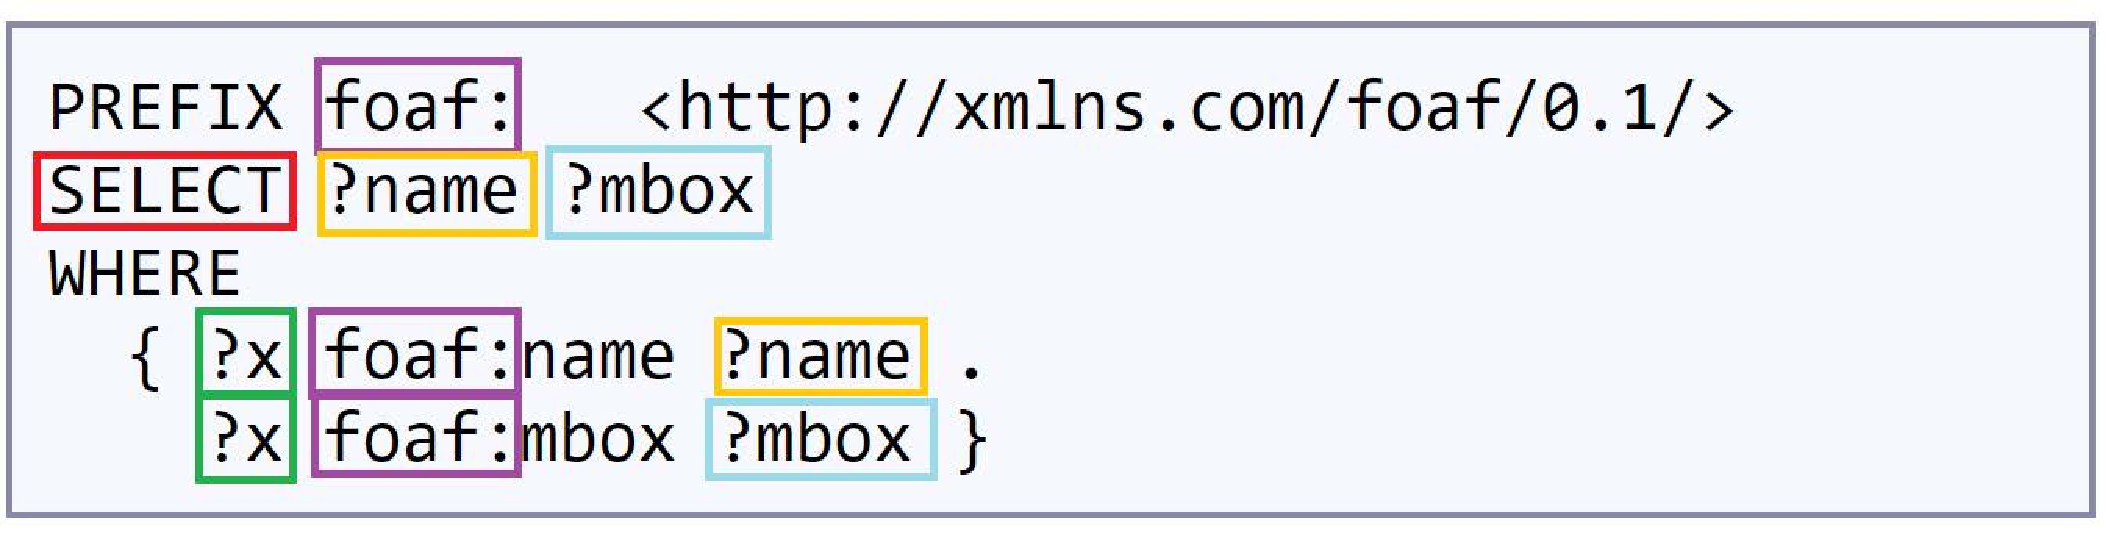
\includegraphics[width=1\textwidth]{figures/sparql-example.pdf}
    \caption{SPARQL query with highlights}
    \label{fig:sparql-example}
\end{figure}

\begin{figure}[H]
    \centering
    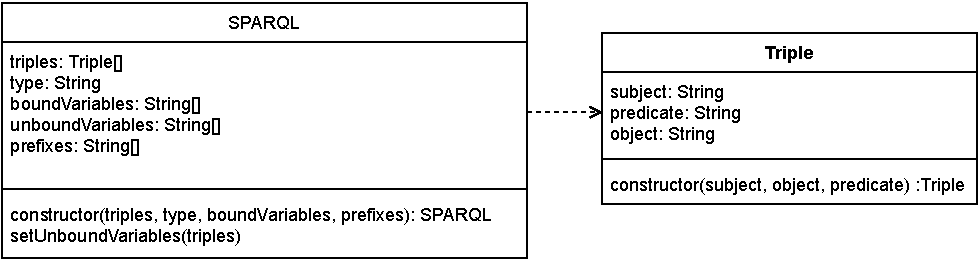
\includegraphics[width=1\textwidth]{figures/SPARQL-Triple-class.pdf}
    \caption{Class diagram for SPARQL}
    \label{fig:SPARQL-Triple-class}
\end{figure}

As it can be seen in figure \ref{fig:SPARQL-Triple-class}, a couple of different variables are defined for the SPARQL class. First is the Triple array. This array contains all the “triples” in the query. Triples are normally reserved for RDF, but the principle can be used in SPARQL as well, in which they are called graph patterns. An example of a graph pattern in a SPARQL query could be “?x foaf:name ?name”, which can be found in the WHERE section of the query, see figure \ref{fig:sparql-example}. A triple therefore consists of three strings: a subject, a predicate, and an object. Next is the type of the query, which can be SELECT, CONSTRUCT, DESCRIBE, and ASK, but for the current version of the program only SELECT is implemented. Bound and unbound variables can be found in the triples as well, but the difference is that bound variables are included in the top of the query next to the type. Regarding figure \ref{fig:sparql-example}, the bound variables are the variables the user wants to select. Lastly the prefixes are stored in an array.

\subsection{Textual parser}
 When it comes to the textual parser the goal of the first iteration is familiarising ourselves with the concepts of a parser. The entire idea of a parser is taking some text and figuring out patterns to allow for the software to return some data based on what is written, in our case we want to be able to write a SPARQL query and convert it to the SPARQL object we have created so we can share the information between the visual and textual parts. To keep this as simple as possible we wanted to do this with already known easy to under technologies. The first challenge is to figure out how we get text to something readable for the software, then we have to figure how are we going to match the text to a pattern we expect to see and lastly how are we going to convert from the textual pattern to an object and from an object to the textual pattern
 
\subsection{First design}
Based on the requirements in the previous chapter and the class diagram in figure \ref{fig:SPARQL-Triple-class}, a complete system design is created, see figure \ref{fig:initial-design}. The design is primarily based on the must have requirements. Starting on the side of the visual part, a visual handler and a visual parser has been added. The job of the visual handler is to control the visualisation. This means it will handle requirements such as node creation and arrow creation. The visual handler has a two-way connection with the visual parser. The visual parser gets the visualisation from the visual handler by a call of the “getVisualisation” method. This returns a set of SVG elements, which the visual parser shall convert to a SPARQL object and send to the textual parser. The conversion between SVG elements and SPARQL object shall be done by taking any textual attributes in the visualisation and append them as the triples of the SPARQL object. The textual parser shall then take the SPARQL object and convert it to one string for the textual handler, which will update the text field on the page. The text field will be for query writing and is correlated to the requirement of the similar name: Writable query. This entire process of converting it from a visualisation to a SPARQL object, and then a text string shall be reversed so a two-way relationship can occur. This corresponds to the functional requirement “Visual and textual updating”.

\begin{figure}[H]
    \centering
    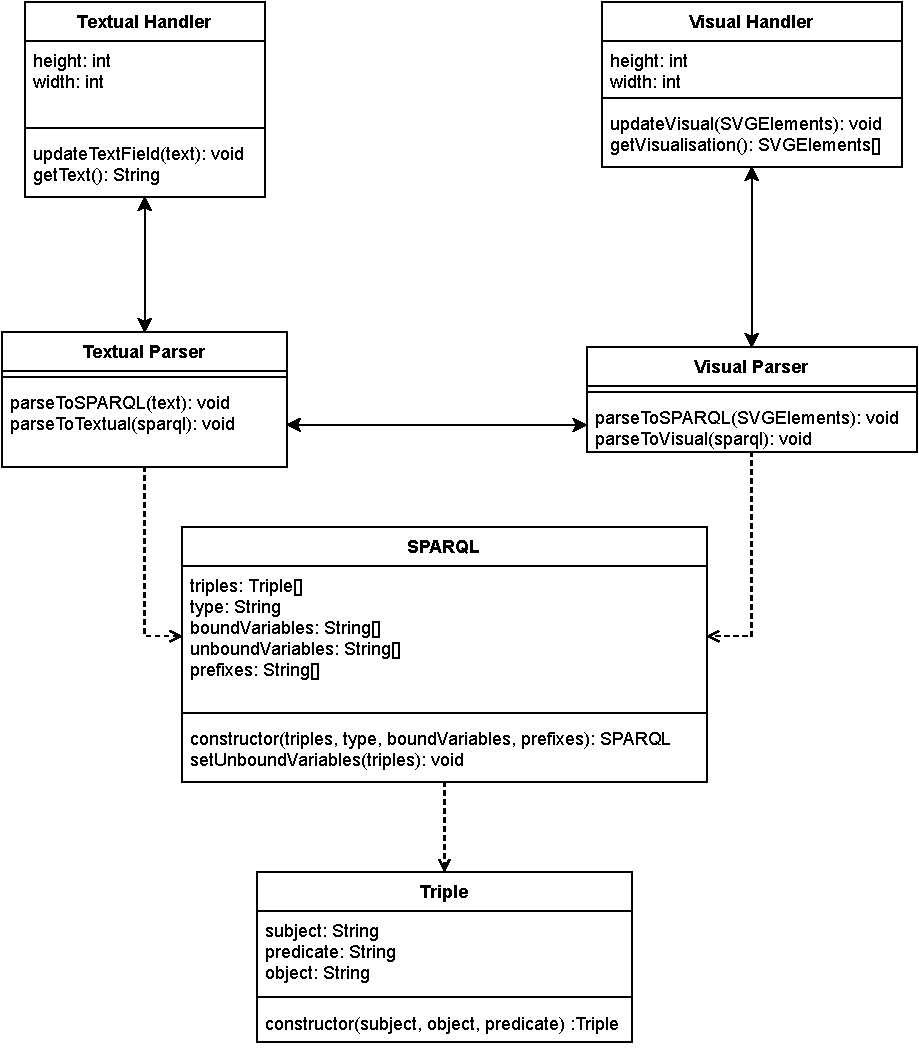
\includegraphics[width=1\textwidth]{figures/initial_design.pdf}
    \caption{The first design}
    \label{fig:initial-design}
\end{figure}

\subsection{Actual design}
During implementation, some complications arose with the initial design. The main issue was the conversion from visual handler to visual parser. In the first design, an array of SVG elements was sent to the visual parser. This was troublesome as it is difficult and very code heavy to extract the text attributes from the array and figure out where they belong. Therefore, a new design was created, figure \ref{fig:first-design}, in which the two classes Arrow and Node have been added. These classes both contain the relevant SVG for creating their visualisation, and act as a datatype which can be transferred between the visual handler and the visual parser. As the arrow class represents a graph pattern, a conversion can be made simply by sending the array of arrows in the visualisation.

\begin{figure}[H]
    \centering
    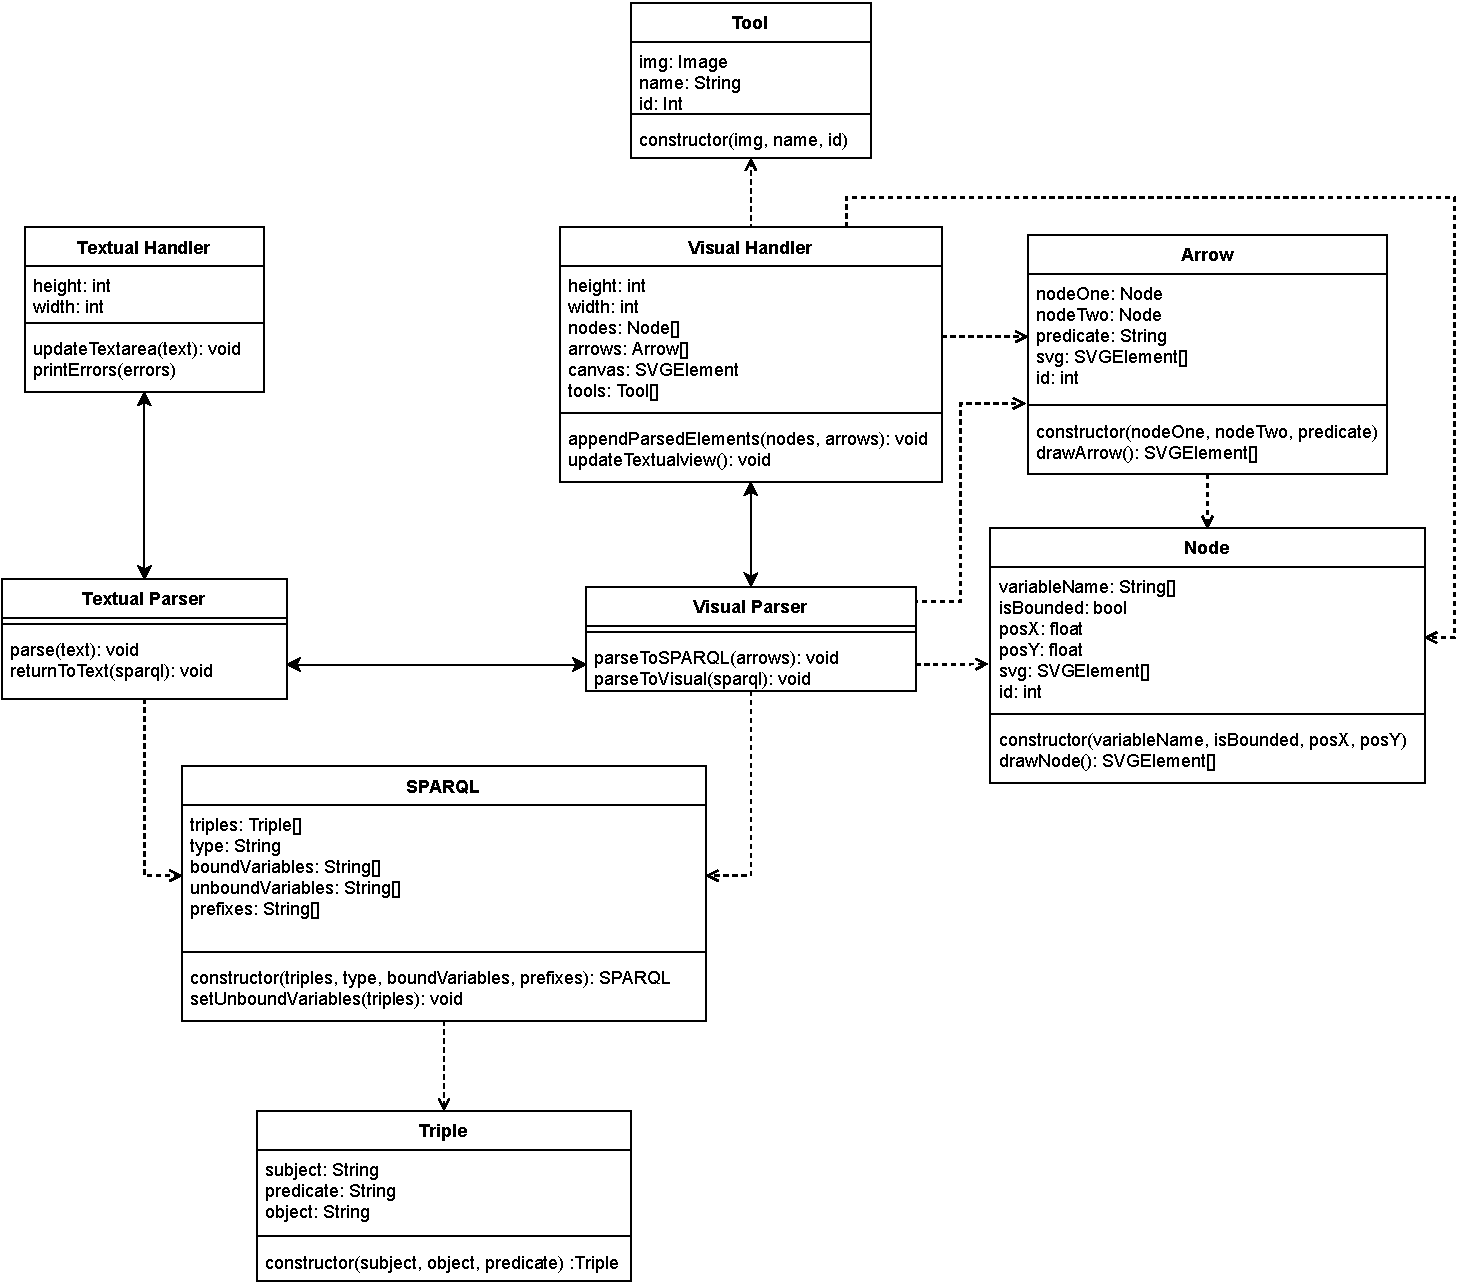
\includegraphics[angle=90,origin=c,width=1.3\textwidth]{figures/1st_iteration_design.pdf}
    \caption{The actual design}
    \label{fig:first-design}
\end{figure}

\subsection{SPARQL visualised}
In the requirements section it is stated that the visualisation shall be made from nodes and arrows, but first the nodes and arrows must be specified to know what they contain and what they resemble. As mentioned earlier in the chapter, SPARQL utilises sets of triple patterns, a graph pattern, to construct queries. These triple patterns mimic the RDF triple pattern of a subject, predicate, and object, and can be substituted for variables in the queries.

\bigskip
Looking at the SPARQL query in figure \ref{fig:sparql-example}, the most important parts of the query have been highlighted. The purple boxes highlight a prefix, in this case foaf, red highlights the type of query, select, yellow and blue boxes represent variables, and green boxes for the subject. All the highlights are however not necessarily node worthy in the visualisation. As an example, the type of query is not needed as a node but perhaps an option on the side.

\bigskip
A couple of suggested UI designs, which can lead to multiple combinations, can be seen in appendix {\color{red}x.x}. These designs are directly correlated with figure \ref{fig:sparql-example}, meaning the colours are the same. This relates to the requirement “Query and node highlighting”. The requirement “Select different queries” has two options. Either it shall be a node connected to the bound variables or a selection outside of the canvas. This is doable as the possibilities are limited to 4: Select, Construct, Ask, and Describe. The advantage of using the node form is that it is easily visible which variables are the bound variables. However, there is also room for confusion both in code and visually. New users might think that the type node is a part of a triple. Code wise, it is important to distinguish between the different types of nodes, as it is important not to convert it to a triple. As it can be seen in figure \ref{fig:chosen-ui}, which is the final choice of visualisation, the choice fell on the type selection disconnected from the canvas. This was because it should already be possible to see the bounded variables by their colour, while the disconnect avoids confusion.

For the arrows between the nodes, the selection came between an arrow with a name above or yet another node with a name. The second solution did however not make any sense and was more confusing than helpful. It was therefore decided to just use arrows as it can be seen in figure \ref{fig:chosen-ui}.

\begin{figure}[H]
    \centering
    \includesvg[width=1\linewidth]{figures/UI_idea_1.svg}
    \caption{The chosen UI for the visualisation}
    \label{fig:chosen-ui}
\end{figure}


\section{Implementation}
\subsection{Visual implementation}
For the first iteration, the visual implementation had to have the following features:
\begin{itemize}
    \item A canvas with node creation and manipulation.
    \item A two-way conversion between SPARQL objects and the visualisation.
\end{itemize}
This led to the following solution, figure \ref{fig:visual-ui-first}.

\begin{figure}[H]
    \centering
    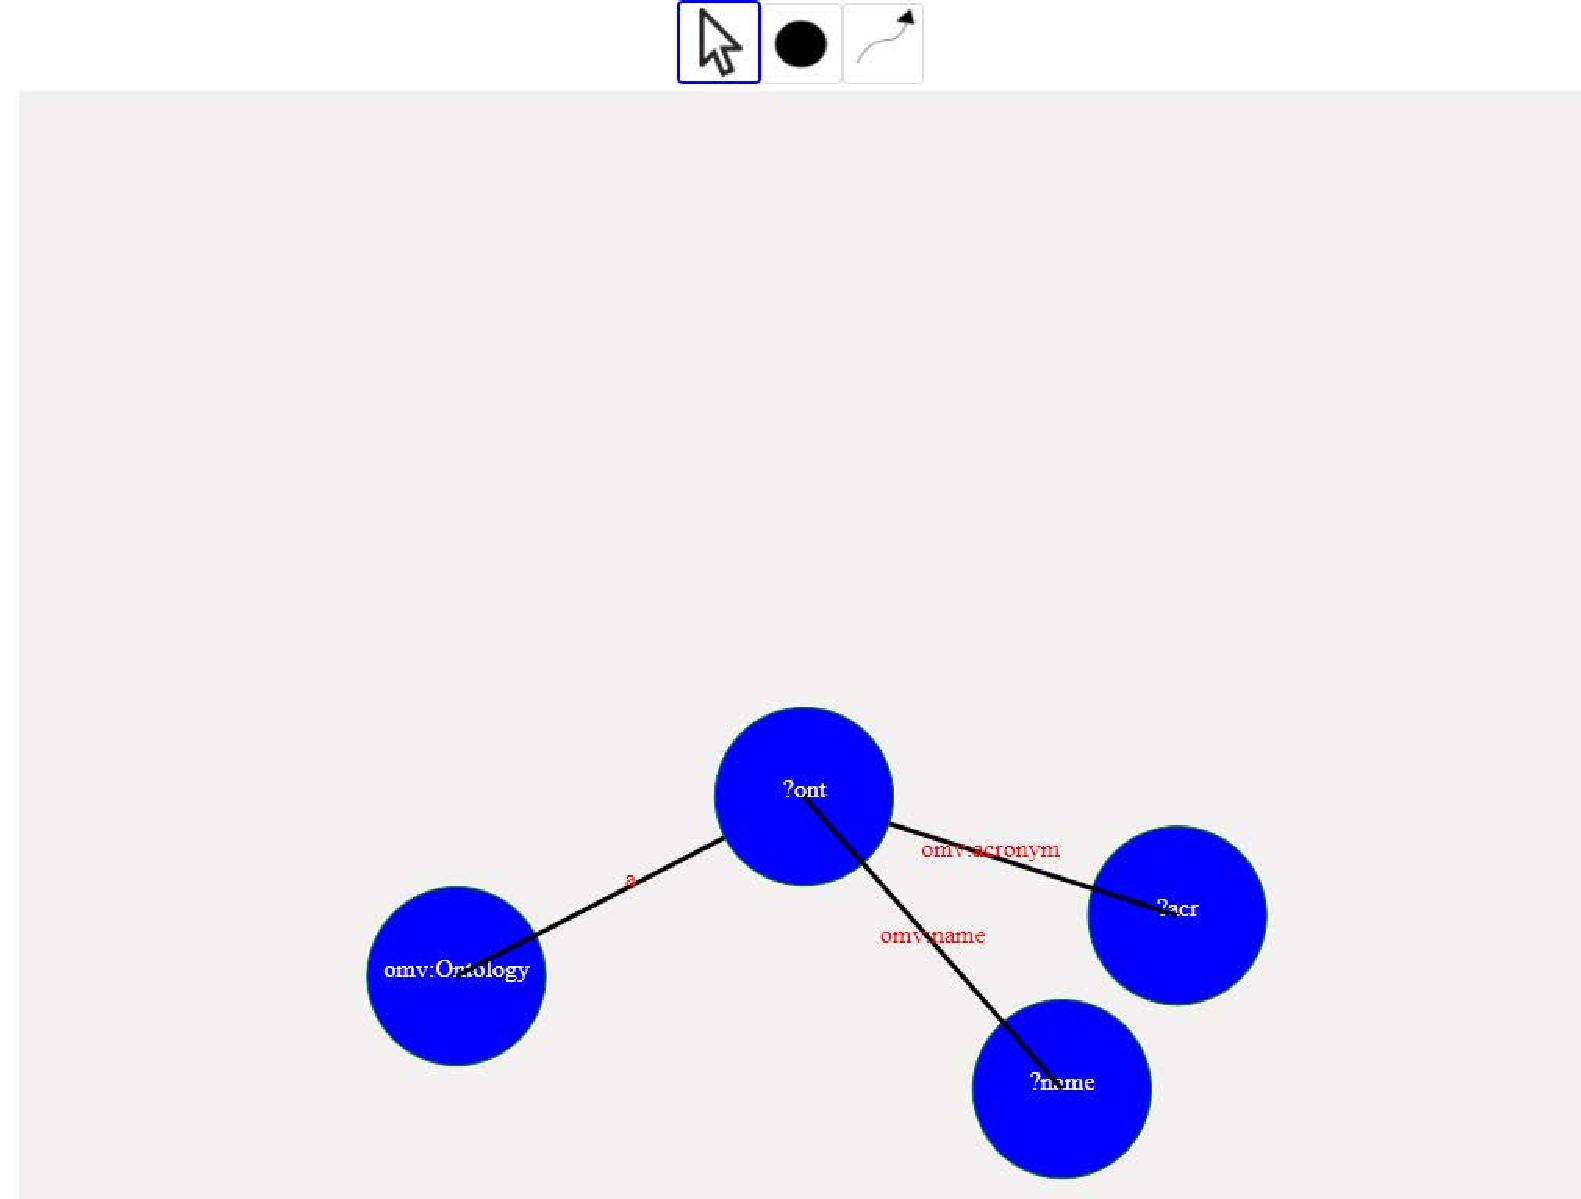
\includegraphics[width=1\linewidth]{figures/visual-ui-first.pdf}
    \caption{Snippet of the visual part of the program.}
    \label{fig:visual-ui-first}
\end{figure}
The figure above shows the visualisation of a simple SPARQL query. As discussed in the design segment, each node represents a variable, subjects and objects, and the lines between are the predicates of the graph pattern. Above the canvas, which is the grey area surrounding the nodes, three different tools are shown. The first tool is for selecting nodes and lines, which can then be deleted from the visualisation. The second tool is for node creation and the third is for line creation. Figure \ref{fig:visual-arrow-node} shows the popups created from the last two tools.

\begin{figure}[H]
    \centering
    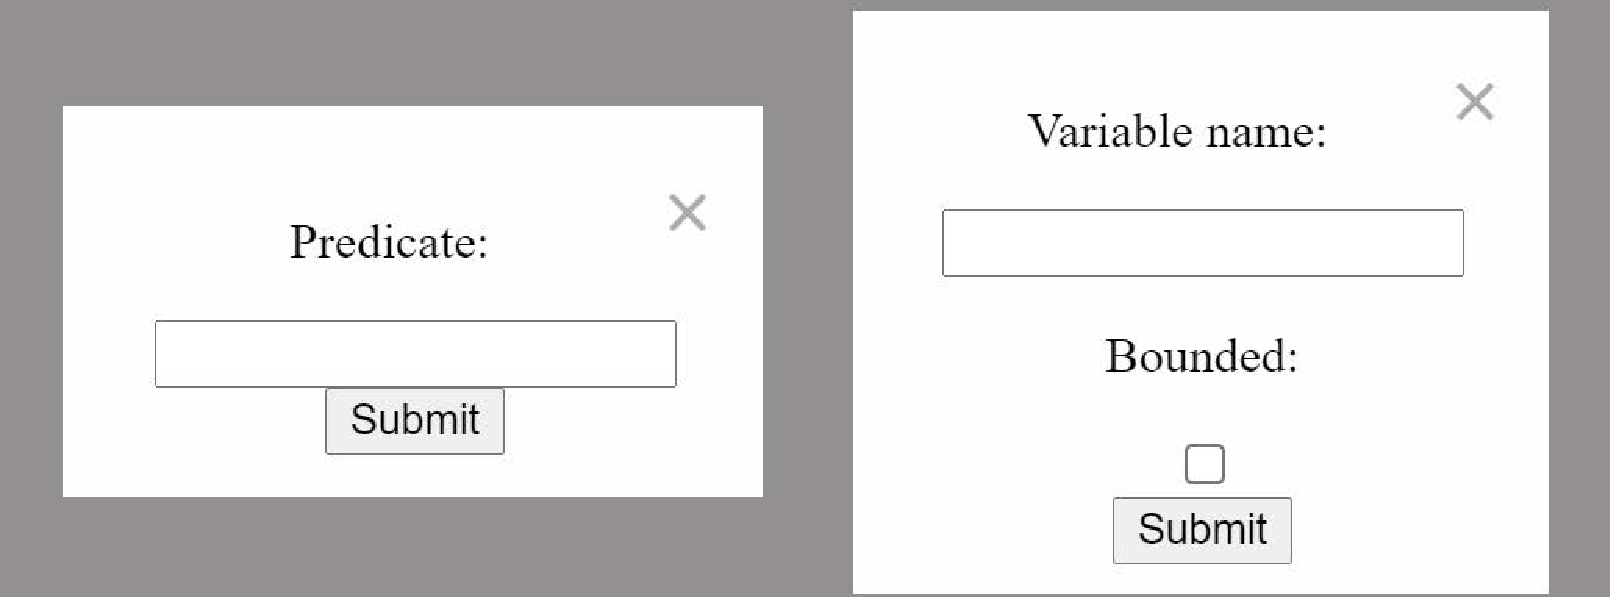
\includegraphics[width=1\linewidth]{figures/visual-arrow-node.pdf}
    \caption{Left is the line tool popup, right is the node creation tool popup.}
    \label{fig:visual-arrow-node}
\end{figure}

\subsection{Force directed spring graph layout}
While it is difficult to see in figure \ref{fig:visual-arrow-node}, the visualisation is affected by forces which have an impact on node positions and the lengths of the lines. This helps the visualisation commit to a spring graph layout without overlaps in nodes. This was implemented using the following algorithm, figure \ref{fig:algo}:
\begin{figure}[H]
    \centering
    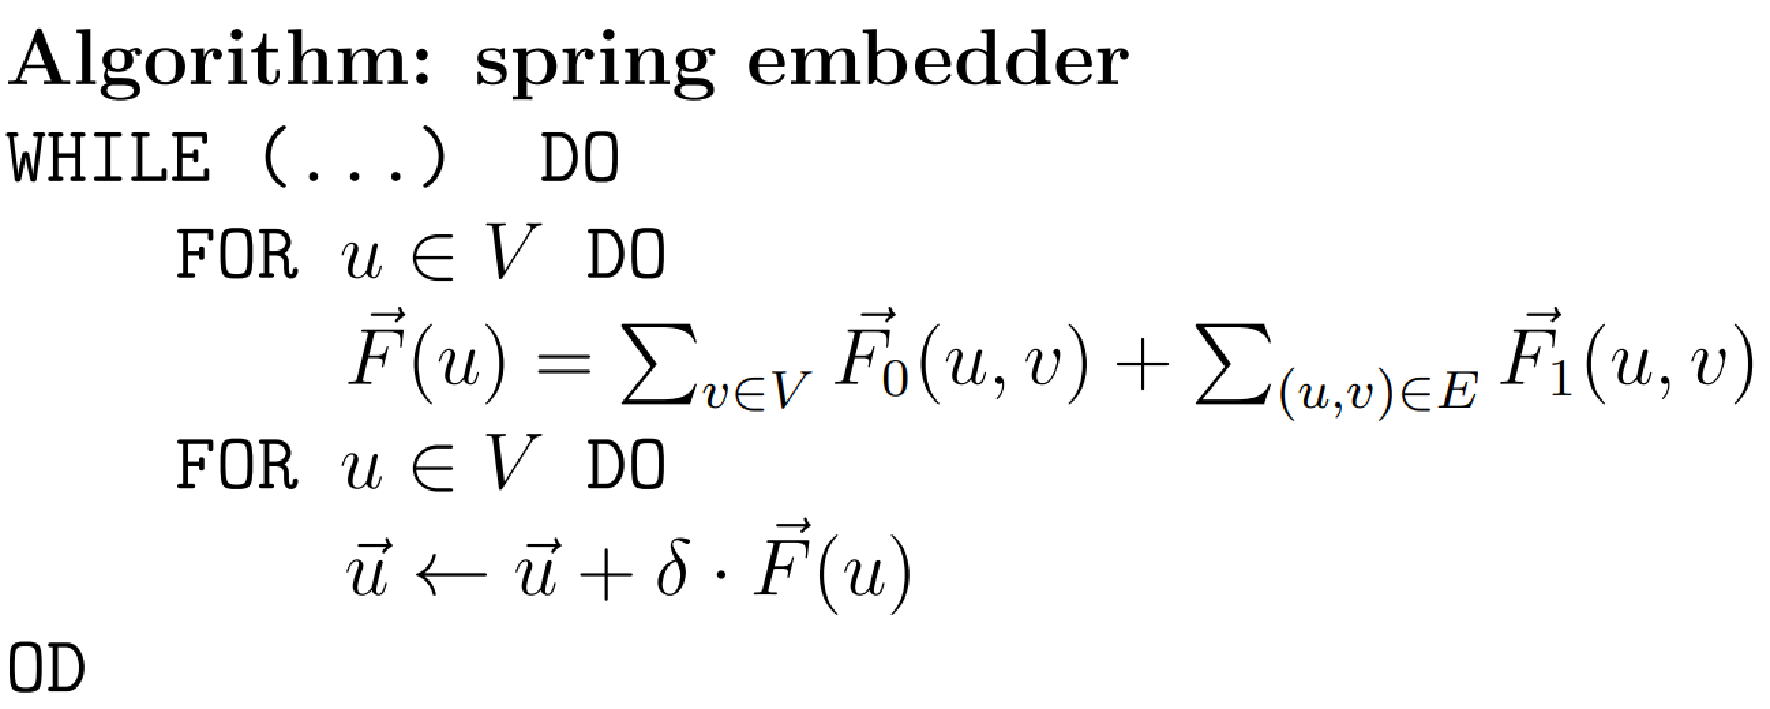
\includegraphics[width=1\linewidth]{figures/algo.pdf}
    \caption{Algorithm for a spring graph layout from Praktikum Algorithmen-Entwurf}
    \label{fig:algo}
\end{figure}
The algorithm takes a given graph with the vertices V, nodes, and edges E, arrows. Then for each vertex two combined forces are applied. The first force acts as a repulsive force between the vertices and will separate the vertices from each other. The second force is the force of the edges. The job of an edge is to hold two vertices together and therefore the force is counteracting the initial repulsive force of the vertices. A second for loop then applies the force to the position vectors of the vertices. This algorithm is meant to run while the combined forces are not equal to zero. However, zero can be a difficult value to hit exactly and the algorithm can therefore be run in several iterations or until the combined force is within a certain threshold. In this implementation, the algorithm runs until the force is within the range {-1,1}.

\subsection{Textual implementation}
The parser in the first iteration worked based on “if statements” and simply looking if the next character in the text was the character that was expected and if not print an error citing where and what the error was. This was a decent enough approach to get something that works but it was not great for maintaining as the potential for bugs was very high since any tiny error on our end would break the entire system or if the user used slightly different spacing than what was expected it could potentially also break fx. a double space instead of a single space. The use of a series of if statements is also very inefficient which for our relatively small scale and beginner friendly prototype is not the biggest concern as it does not scale well. Another issue with doing it this way is that implementing a new type or other new features would require one to check everywhere to make sure nothing broke and not only the part that was changed/added meaning that the code could not really be reused for multiple different types/inputs\\
To look at a code example of how this long list of if-statements worked see figure \ref{fig:textual-parser}.
\begin{figure}[H]
    \centering
    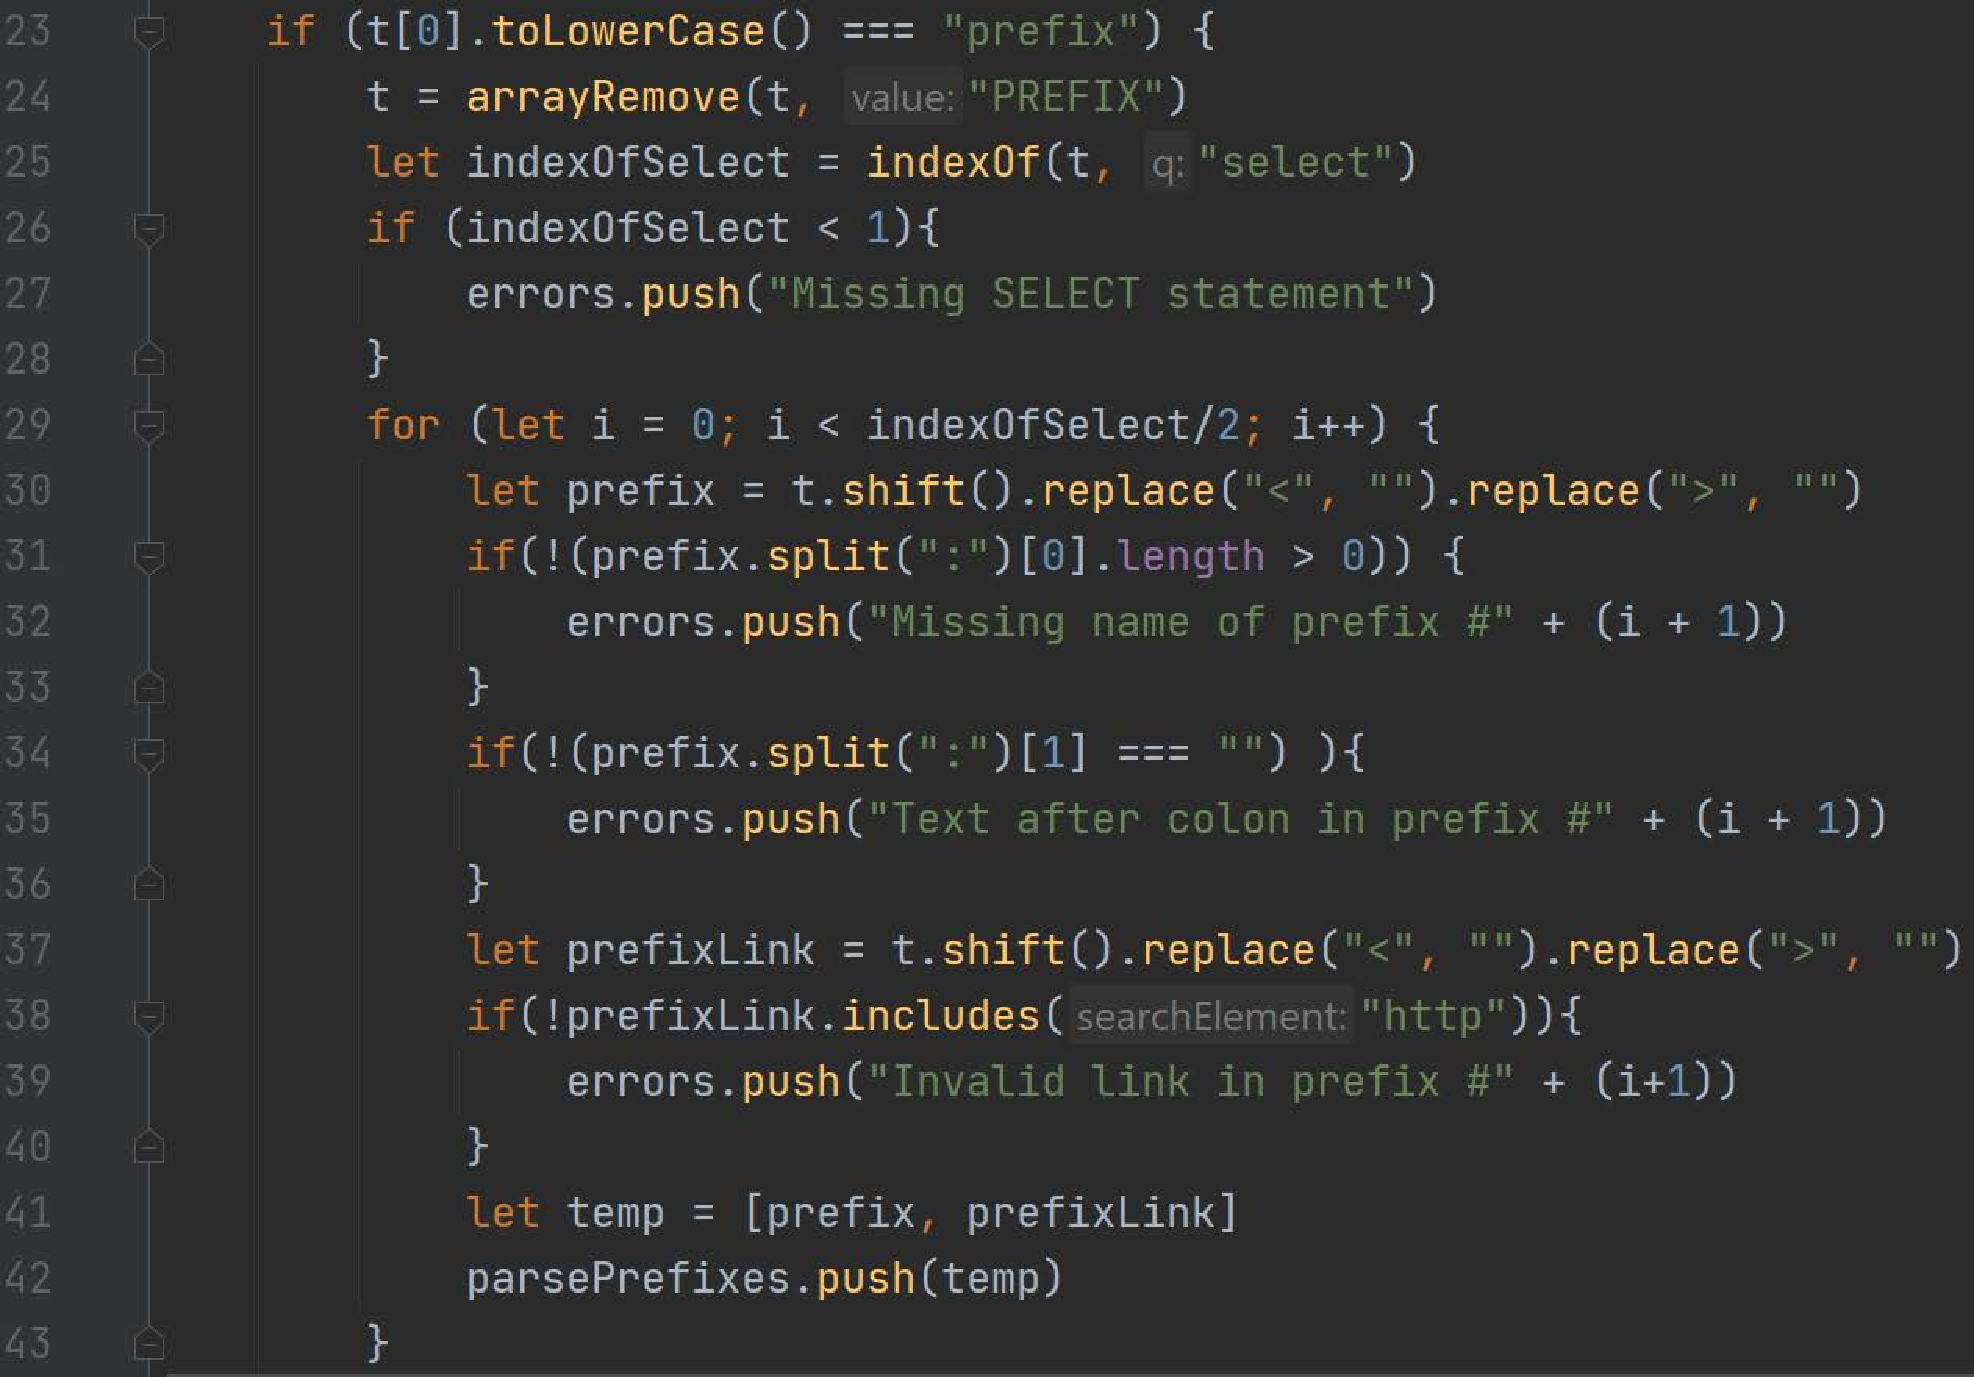
\includegraphics[width=1\linewidth]{figures/textual-code-first.pdf}
    \caption{Code example from the textual parser}
    \label{fig:textual-parser}
\end{figure}
The first step was to look at if the first character was the word “prefix” this was done to determine if the user had any prefixes in their query so we could handle these first. The next step was to remove all the instances of the word prefix as we do not care about those anymore, then we get the index of the “select” keyword meaning when the user’s last prefix is done. A quick check to make sure the word select was found or else we could make an error to say that it is missing. The next step is to run through each prefix and get the name and link so we can add them to the SPARQL object in the end. To do this we decided on first removing the angular brackets as these would just potentially mess with the names, then we checked is there a name of the prefix included and if not create an error saying that there is no name in this prefix, then we had to ensure there was no text after the colon in the prefix as a prefix is defined as a name ending with a colon. The last step was to make sure that the link included was valid and then push it to the prefixes array.

\section{Evaluation}
The first iteration had lived up to the given requirements, but the solution was subpar. As the whole visualisation was created only using vanilla JS and SVG, algorithms connected to graph theory had to be entirely implemented by the group. This meant that while functional, the look of the program became harsh looking. The force directed graphing moved the nodes into the right positions, but the translation of the nodes was not smooth. The nodes and lines were overlapping depending on which element had last been added, and while this is fixable, the solution will probably lead to a less than practical approach.

The textual parser was also not without its flaws, the biggest issue we ran into was the problem of code extension, the parser was built so specific to handle one case that any extension of the code would require an almost full rewrite. The parser also struggled with error handling as this was hand made meaning that any error we did not think of would break the system there was no automatic “unexpected character” or anything similar. The last three majors were all due to the way we decided to implement the checks for whether a pattern matched, the implementation choice of using if-statements seemed like a good idea at the start since it was a known and simple technology, later it would prove to cause issues with performance, maintainability, and readability. The performance was due to having to check each word whether it matches a long series of patterns, the maintainability issues was due to having to decipher these long pattern matches made it almost impossible to edit without breaking something elsewhere. The issue of readability matches closely with the issues of maintainability since the long pattern matches were almost impossible to read and understand even to the point where it was hard for the others in the group to understand what was going on.